%17/02 - Aythami Morales 
\chapter{Aprendizaje no supervisado - Clustering}
\section{Clustering}
En el \textbf{aprendizaje supervisado}, se dispone de etiquetas (valores de $y$) que permiten medir el rendimiento del modelo. En cambio, en el \textbf{aprendizaje no supervisado}, no se tienen etiquetas, y el objetivo es descubrir patrones o estructuras ocultas en los datos. Una de las técnicas más comunes es el \textbf{clustering}, que agrupa los datos en función de sus características o similitudes.

El clustering se basa en la \textbf{proximidad} entre datos o ítems. Esta proximidad puede medirse de diversas formas, dependiendo del tipo de datos y del problema:
\begin{itemize}
\item \textbf{Distancia euclídea:} La distancia más corta entre dos puntos en un espacio euclídeo.
\item \textbf{Distancia de Hamming:} Utilizada en datos binarios, mide el número de bits que difieren entre dos vectores.
\item \textbf{Distancia de Manhattan:} Mide la distancia entre dos puntos moviéndose solo en direcciones horizontales o verticales (no en diagonal).
\end{itemize}

En casos más complejos, como con palabras o distribuciones estadísticas, la proximidad puede medirse utilizando técnicas avanzadas, como las empleadas en modelos de lenguaje (LLMs) o métricas específicas para distribuciones.

\subsection{Definición de Clustering}
El clustering es la organización de una colección de patrones en grupos (clústeres) basados en su similitud (Jain, Murty, et al. 1999). Mientras que clustering es aprendizaje no supervisado, la clasificación sí lo es, ya que se utilizan las etiquetas de los datos para, a datos nuevos, asignarles esas etiquetas. Un clúster puede definirse como:
\begin{itemize}
\item conjunto de objetos similares.
\item un grupo de puntos donde la distancia entre dos puntos del mismo clúster es menor que la distancia entre cualquier punto del clúster y cualquier punto de otros clústeres.
\item regiones densamente conectadas en un espacio multidimensional separadas por puntos o regiones poco conectados.
\end{itemize}

\subsection{Distancia}
La distancia entre dos instancias $x^{(i)}$ y $x^{(j)}$ es una métrica si satisface las siguientes propiedades:
\begin{enumerate}
\item \textbf{Desigualdad triangular}
$$d(\vec{x}^{(i)}, \vec{x}^{(j)}) \leq d(\vec{x}^{(i)}, \vec{x}^{(k)}) + d(\vec{x}^{(k)}, \vec{x}^{(j)}), \forall  \vec{x}^{(i)}, \vec{x}^{(j)}, \vec{x}^{(k)} \in \mathbb{R}^n$$

\item \textbf{Identidad de los indiscernibles}
$$d(\vec{x}^{(i)}, \vec{x}^{(j)}) = 0 \rightarrow \vec{x}^{(i)} = \vec{x}^{(j)}, \forall \vec{x}^{(i)}, \vec{x}^{(j)} \in \mathbb{R}^n$$
\end{enumerate}

\section{Algoritmo K-means}
K-means es uno de los algoritmos más utilizados en clustering. Su objetivo es dividir un conjunto de datos en $K$ clústeres, donde cada dato pertenece al clúster cuyo centroide (punto central) está más cerca.

\subsection{Pasos del algoritmo K-means}
\begin{enumerate}
\item \textbf{Inicialización}: Se elige el número de clústeres $K$. Se inicializan $K$ centroides de forma aleatoria.
\item \textbf{Asignación}: Cada dato se asigna al clúster cuyo centroide está más cerca (según una métrica de distancia, como la euclídea).
\item \textbf{Actualización}: Se recalcula la posición de cada centroide como el promedio (centro de masas) de todos los datos asignados a su clúster.
\item \textbf{Iteración}: Los pasos de asignación y actualización se repiten hasta que los centroides ya no cambian significativamente.
\end{enumerate}

\begin{figure}[h]
\centering
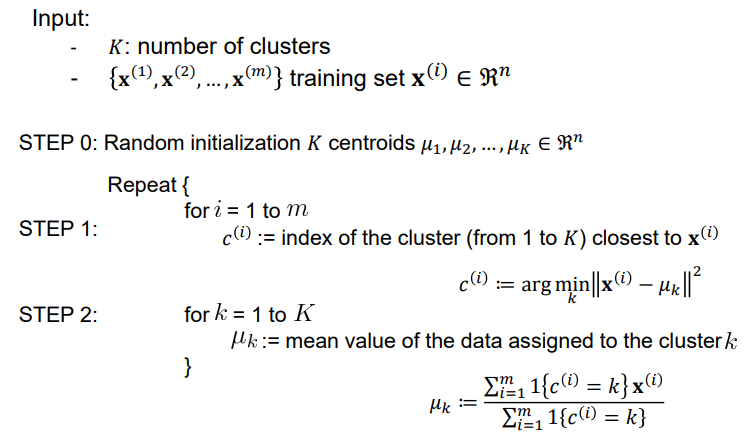
\includegraphics[width = 0.7\textwidth]{figs/kmeans-algorithm.png}
\end{figure}

\subsection{Inicialización aleatoria y óptimos locales}
La inicialización aleatoria de los centroides puede llevar a soluciones subóptimas. Para mitigar esto, se pueden utilizar técnicas como:
\begin{itemize}
\item \textbf{Inicialización basada en datos}: Seleccionar $K$ datos aleatorios como centroides iniciales.
\item \textbf{Repetición del algoritmo}: Ejecutar K-means varias veces y seleccionar la solución con la menor inercia (suma de las distancias al cuadrado entre cada punto y su centroide).
\end{itemize}

Al hacer esto, el algoritmo no es determinista, ya que los resultados no van a ser siempre los mismos, aunque pueda haber resultados más y menos estables. 

\subsection{Superposición entre clústeres}
En algunos casos, los clústeres pueden superponerse, lo que da lugar a clústeres difusos. Por ejemplo, en la clasificación de tallas de ropa (S, M, L), algunos puntos pueden estar en la frontera entre dos clústeres, lo que dificulta su asignación clara.

Cuando no hay tanta separación entre los datos, se pueden dar soluciones dispares. Esto se puede resolver mediante la repetición y medir el rendimiento de las distintas ejecuciones para ver qué solución es la mejor. Se calcula la distancia de cada punto a su centroide y la solución que minimice esa distancia es la que obtiene los centroides más óptimos. 

\begin{figure}[h]
\centering
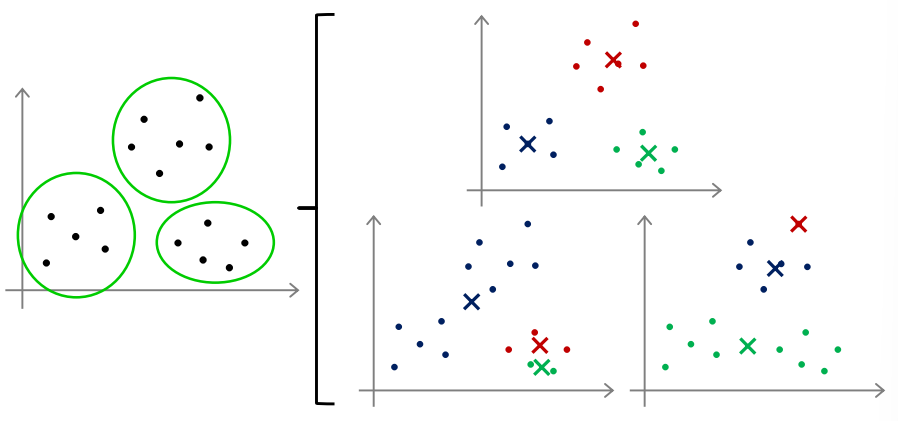
\includegraphics[width = 0.6\textwidth]{figs/kmeans-centroids.png}
\end{figure}

%18/02 - Aythami
\subsection{Función de coste}
K-means no garantiza encontrar el mínimo global de la función de coste, ya que el resultado depende de la inicialización. La función de coste (o función de distorsión) se define como $J$ y tiene el siguiente aspecto:
$$J(c^{(1)}, \ldots, c^{(m)}, \mu_1, \ldots \mu_k) = \frac{1}{m} \Sigma^m_{i = 1} ||\vec{x}^{(i)} - \mu_{c^{(i)}} ||^2$$
donde:
\begin{itemize}
\item $c^{(i)}$ es el índice del clúster al que se ha asignado $\vec{x}^{(i)}$
\item $\mu_k$ es el centroide del clúster $k$ ($\mu_k \in \mathbb{R}^n$)
\item $\mu_{c^{(i)}}$ es el centroide del clúster al que se ha asignado $\vec{x}^{(i)}$. Es una matriz de $m$ elementos.
\end{itemize}

\begin{figure}[h]
\centering
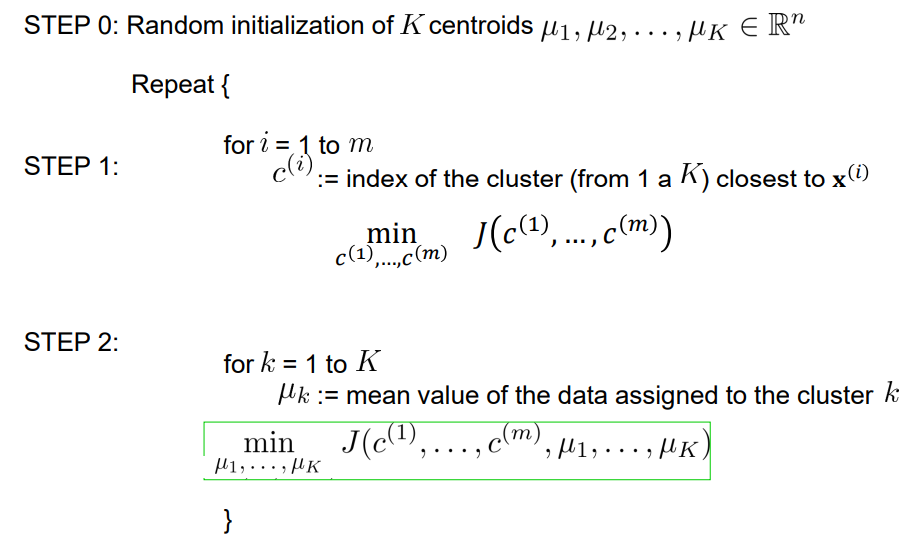
\includegraphics[width = 0.7\textwidth]{figs/kmeans-cost.png}
\end{figure}

Como se ha descrito antes, esto se repite durante varios ciclos para escoger aquel clustering que dé el menor coste.

\subsection{Escoger el número de centroides}
Si el objetivo único es minimizar el coste, la forma de obtener $J = 0$ sería poniendo para cada punto un clúster, pero esto no agrupa los datos según patrones. Por ello, es importante escoger $k$. Si conocemos nuestros datos, podemos saber qué número de $k$ puede ser el óptimo. Otra opción es con el método del codo: se ejecuta el algoritmo de K-means varias veces cambiando $k$ y se ve cuándo la función de coste se ve significativamente reducida. 

\begin{figure}[h]
\centering
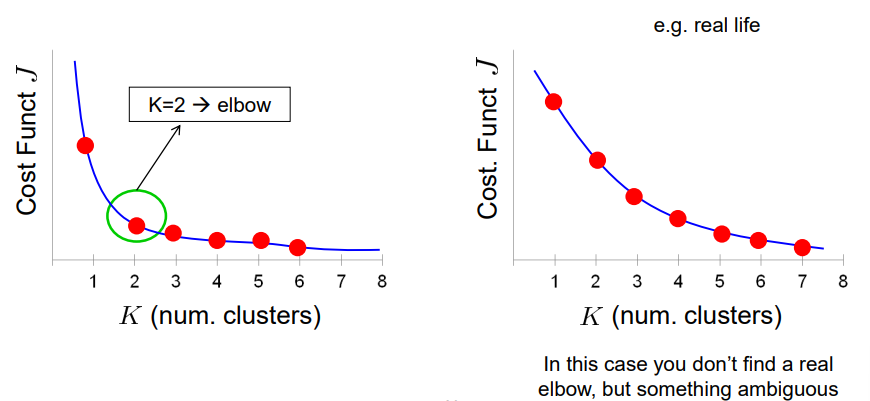
\includegraphics[width = 0.6\textwidth]{figs/kmeans-k.png}
\end{figure}

\section{Bonus track: otros algoritmos}
El algoritmo Gaussian Mixture Models (GMM) permite adaptar los clústers a los datos. De esa forma, en lugar de ser clústeres redondos, se ajustan a la distribución que presenten, pudiendo adoptar otras formas. 